\section*{Justificativa}
A integração entre sistema GSAN com uma ferramenta de PABX será um experimento de cunho prático, realizado para atender a uma demanda do setor de saneamento brasileiro, que atualmente sofre com a dificuldade em fornecer uma comunicação que atenda as expectativas dos clientes através de seu sistema de informação principal.

Com base nas informações disponibilizadas no Relatório de Análise Regulatória da Companhia de Águas de Joinville (CAJ) \cite{AMAE2014} 
situada em no estado de Santa Catarina, divulgado em 2014, demonstra a ineficiência enfrentada pelo setor de saneamento no que diz respeito ao Atendimento ao Público, a companhia considerada universalizada por atender mais 99\% da população urbana com abastecimento de água, somando um total de aproximadamente 508.097 habitantes no município, atualmente enfrenta um número acentuado de reclamações, conforme demonstrado na figura \ref{figura:ligacoesReclamacoes} abaixo:
 

\begin{figure}[H]
	\centering
	\caption{Gráfico da Quantidade de Reclamações Mensais da CAJ} 
	\label{figura:ligacoesReclamacoes}	
	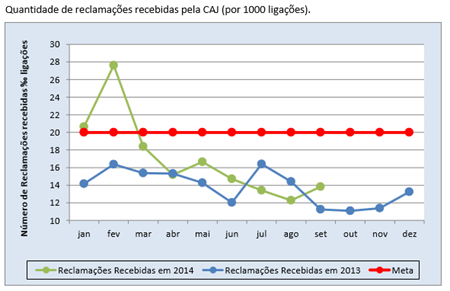
\includegraphics{figuras/LigacoesReclamacoes.png}
	\legend {\fontsize{10}{12}\selectfont {Fonte: \citeonline{AMAE2014}}.}
\end{figure}


 O indicador de Número de Reclamações em 2013 apresentou a média anual de 13,78 reclamações/mil ligações, que reflete na média anual do tempo de espera das ligações que no mesmo ano registrou 75,2 segundos por atendimento. Com uma quantidade notória de reclamações diárias se tornar custoso atender todas solicitações individualmente utilizando somente atendentes sem que haja otimizações nos atendimentos,   deixando evidente o quão necessário se faz adotar medidas para melhorar os sistemas de \textit{Call Center}. 
 
 Conforme informações disponíveis no Sistema Nacional de Informações do Setor de Saneamento (SNIS) \cite{SNIS:2014}, especificamente a Região Norte do país possui um dos piores índices de perda de faturamento do país, consequentemente gera lucros menores e enfrenta dificuldade na ampliação do acesso à população aos serviços de saneamento, dificultando ainda mais investimentos por parte das companhias em tecnologias renovadores para o setor de saneamento.
 
 Visando propor soluções viáveis que possam agregar valor à empresa sem acarretar em custos elevados, utilizando de soluções em software \textit{Open Source} com tecnologias compatíveis, é possível tornar o próprio sistema principal de uma empresa de saneamento o GSAN, capaz de suprir através dos recursos da ferramenta Asterisk, as necessidades de melhoria no atendimento ao público realizado nas Centrais de Atendimento.
 
 Consequentemente favorece a redução de custos e propicia ao cliente final um melhor e mais efetivo relacionamento com a empresa prestadora de serviço.

